\begin{figure} % "[t!]" placement specifier just for this example
	\centering
	\begin{subfigure}{0.35\textwidth}
		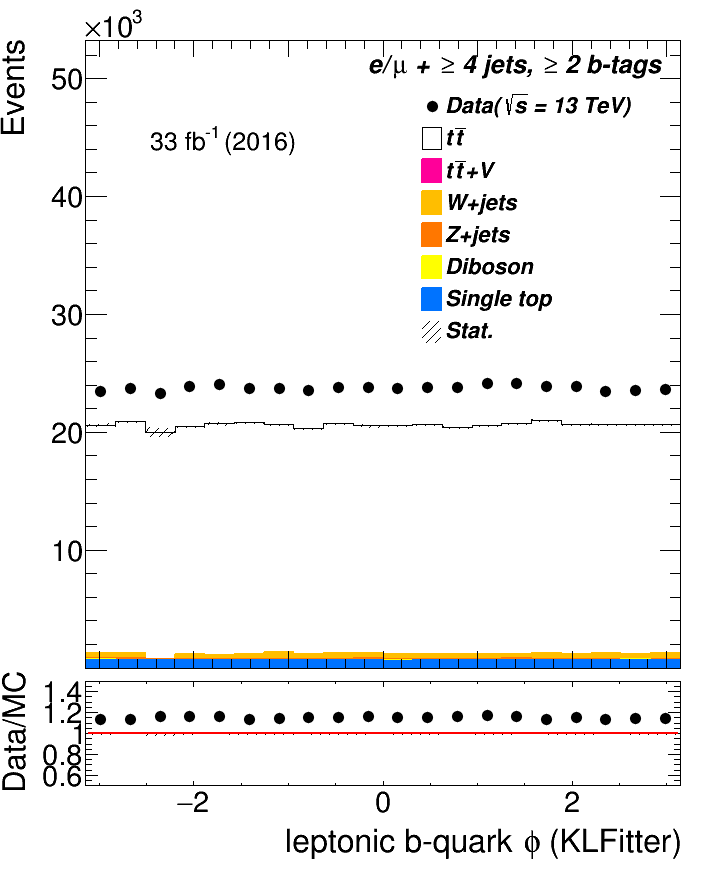
\includegraphics[width=\linewidth]{ControlPlots_emujets_2016_4incl_2incl/klf_blep_phi_emujets_2016.png}
		\caption{$phi$ of the leptonic $b$-jet.} \label{fig:klf61}
	\end{subfigure}
	\hspace*{1.5cm}
	\begin{subfigure}{0.35\textwidth}
		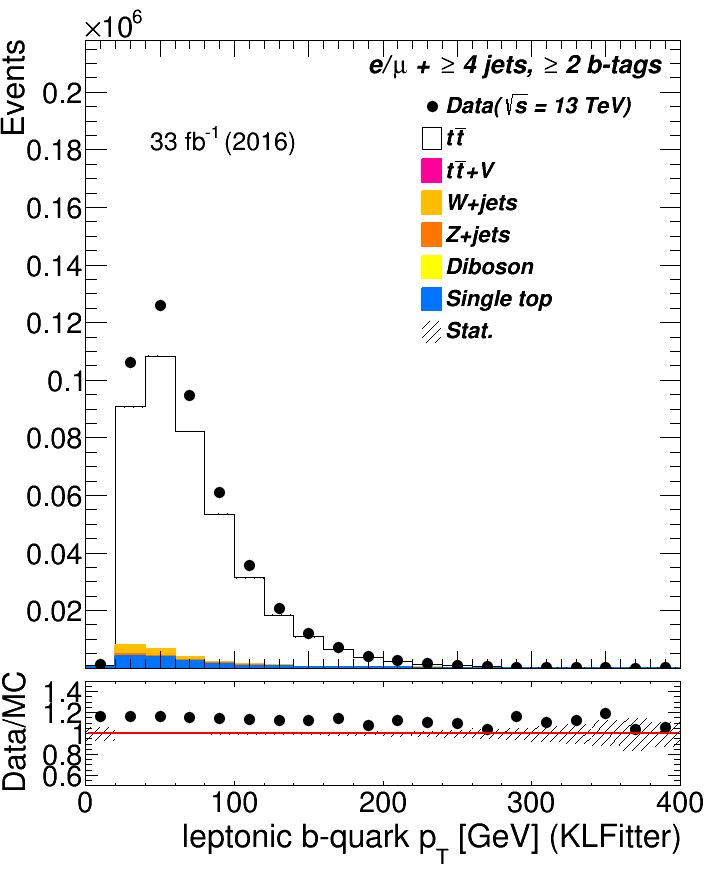
\includegraphics[width=\linewidth]{ControlPlots_emujets_2016_4incl_2incl/klf_blep_pt_emujets_2016.png}
		\caption{Transverse momentum of the leptonic $b$-jet.} \label{fig:klf7}
	\end{subfigure}
	
	\medskip
	\begin{subfigure}{0.35\textwidth}
		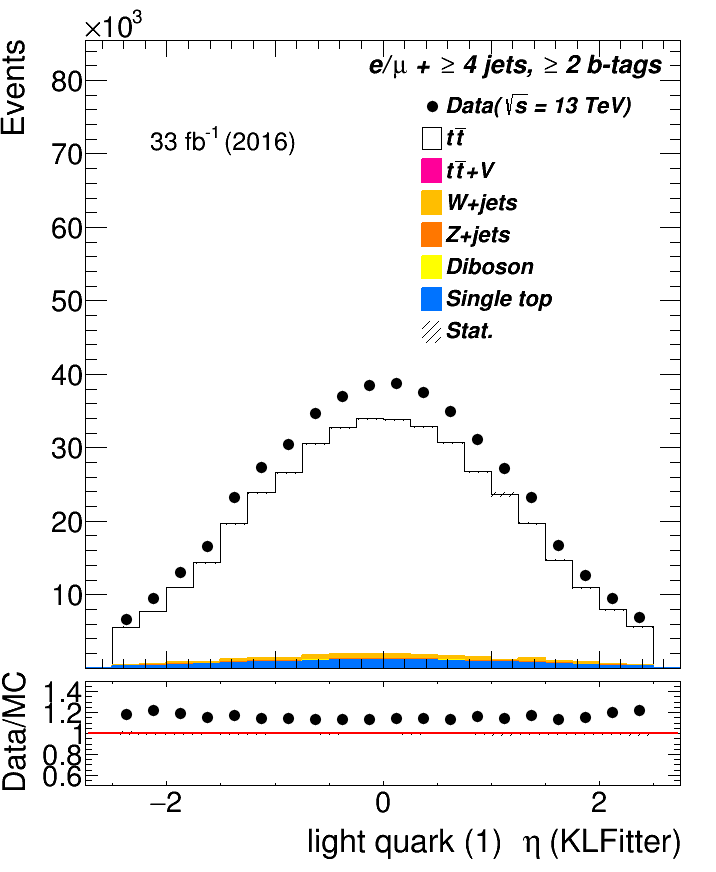
\includegraphics[width=\linewidth]{ControlPlots_emujets_2016_4incl_2incl/klf_lq1_eta_emujets_2016.png}
		\caption{Rapidtiy of the fist light jet.} \label{fig:klf8}
	\end{subfigure}
	\hspace*{1.5cm}
	\begin{subfigure}{0.35\textwidth}
		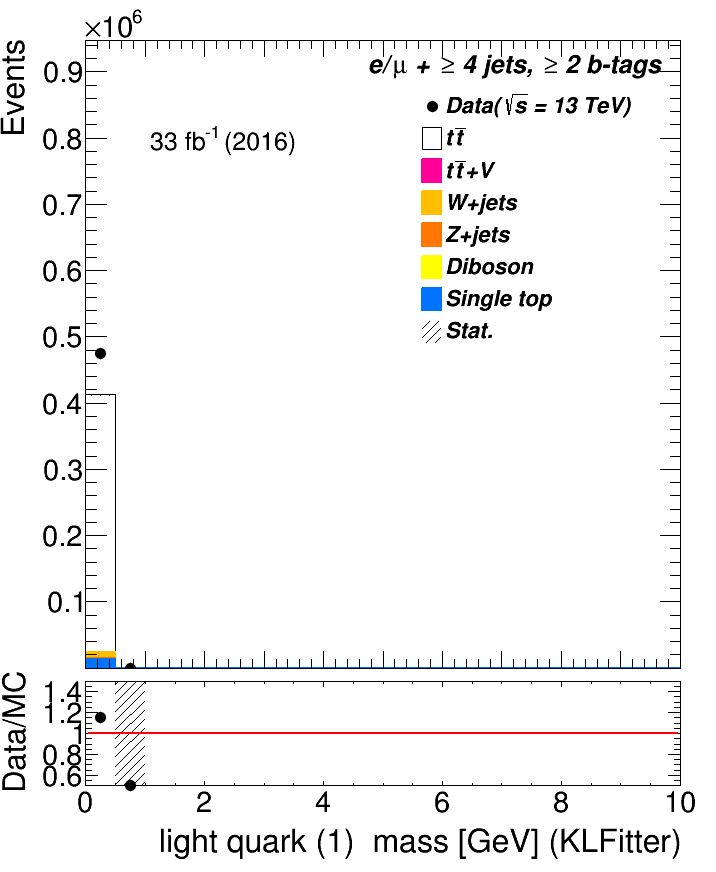
\includegraphics[width=\linewidth]{ControlPlots_emujets_2016_4incl_2incl/klf_lq1_m_emujets_2016.png}
		\caption{Mass of the fist light jet.} \label{fig:klf9}
	\end{subfigure}
	
	\medskip
	\begin{subfigure}{0.35\textwidth}
		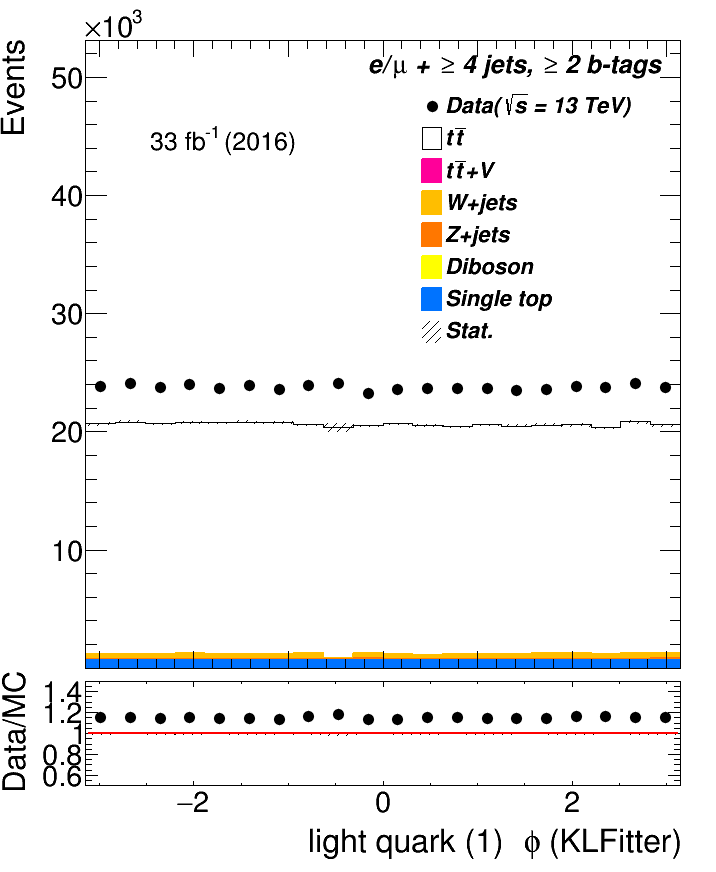
\includegraphics[width=\linewidth]{ControlPlots_emujets_2016_4incl_2incl/klf_lq1_phi_emujets_2016.png}
		\caption{$phi$ of the fist light jet.} \label{fig:klf10}
	\end{subfigure}
	\hspace*{1.5cm}
	\begin{subfigure}{0.35\textwidth}
		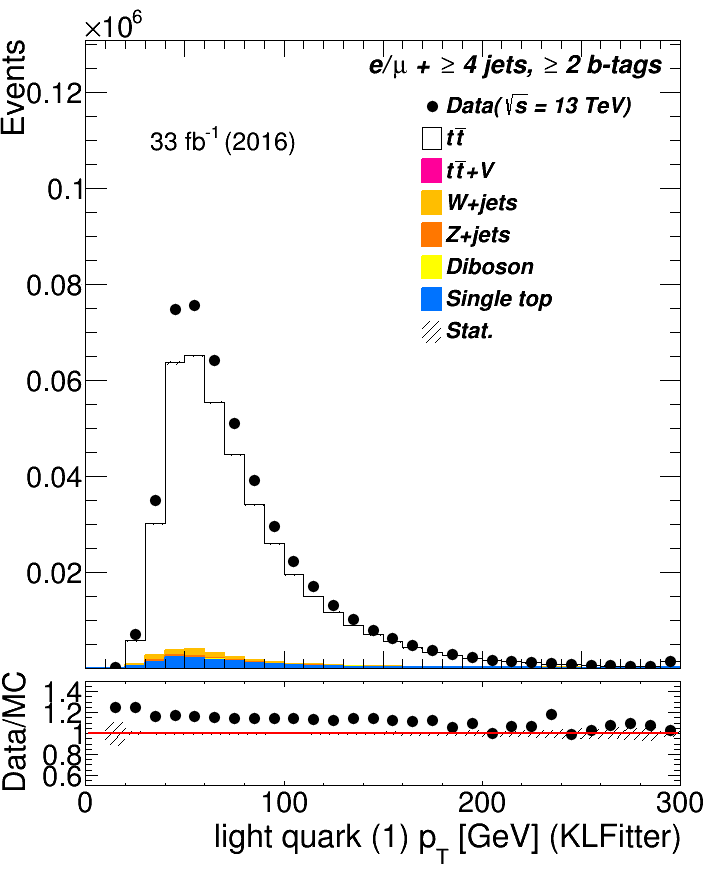
\includegraphics[width=\linewidth]{ControlPlots_emujets_2016_4incl_2incl/klf_lq1_pt_emujets_2016.png}
		\caption{Transverse momentum of the fist light jets. } \label{fig:klf11}
	\end{subfigure}
	\caption{bbbbbbbbbbbbbbbbbbbbbbbbbbbbbbbbbbbbbbbbbbbbbbbbbbbbbbbbbbbbbbbbbbbbbbbbbbb}
\end{figure}	






\begin{figure} % "[t!]" placement specifier just for this example
	\centering
	
	\begin{subfigure}{0.35\textwidth}
		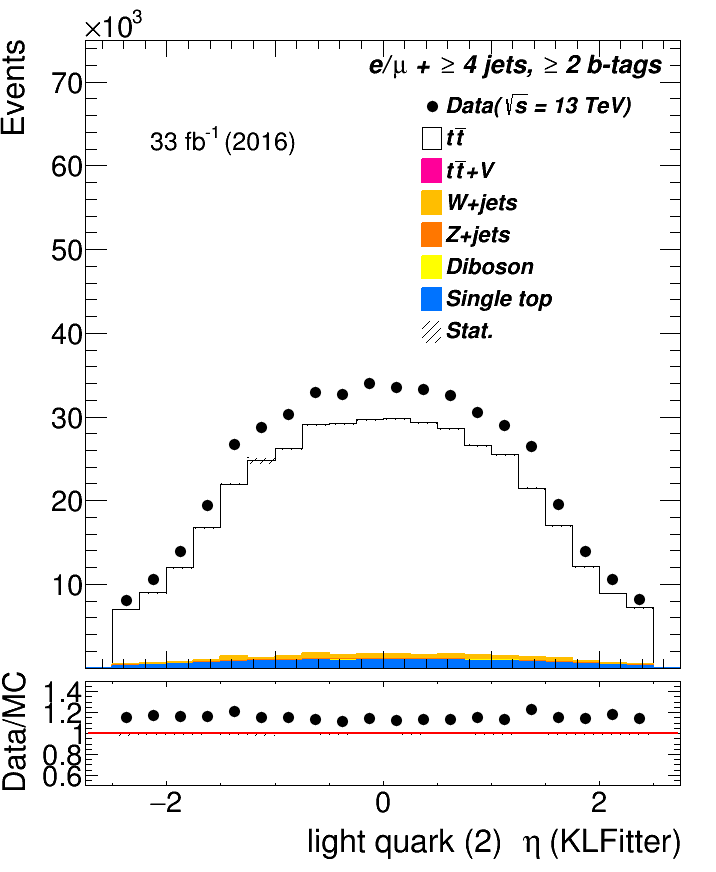
\includegraphics[width=\linewidth]{ControlPlots_emujets_2016_4incl_2incl/klf_lq2_eta_emujets_2016.png}
		\caption{Rapidty of the second light jet.} \label{fig:klf12}
	\end{subfigure}
	\hspace*{1.5cm}	
	\begin{subfigure}{0.35\textwidth}
		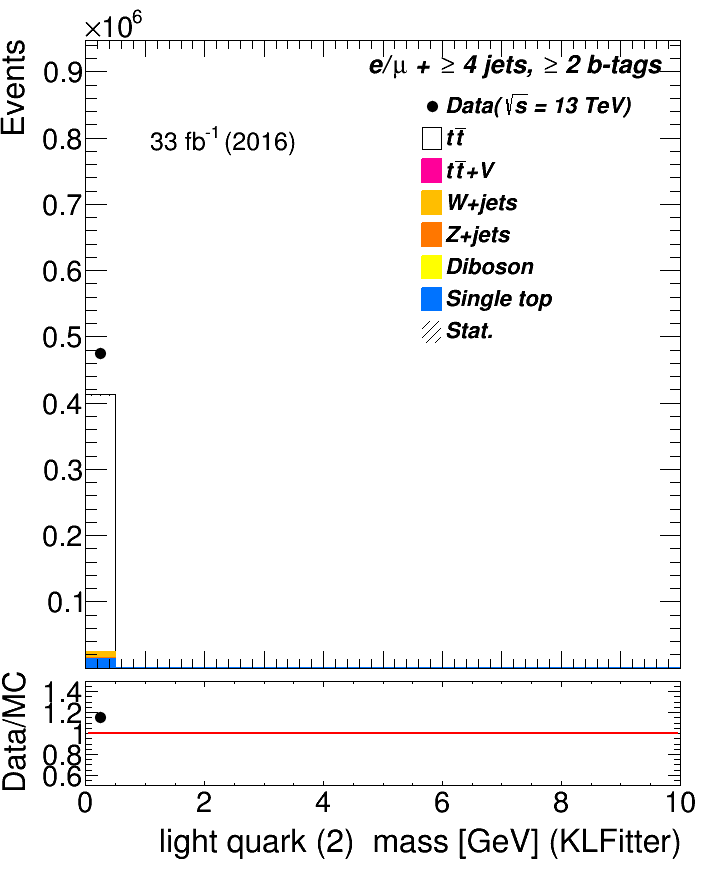
\includegraphics[width=\linewidth]{ControlPlots_emujets_2016_4incl_2incl/klf_lq2_m_emujets_2016.png}
		\caption{Mass of the second light jet.} \label{fig:klf13}
	\end{subfigure}
	
	
	
	\medskip
	\begin{subfigure}{0.35\textwidth}
		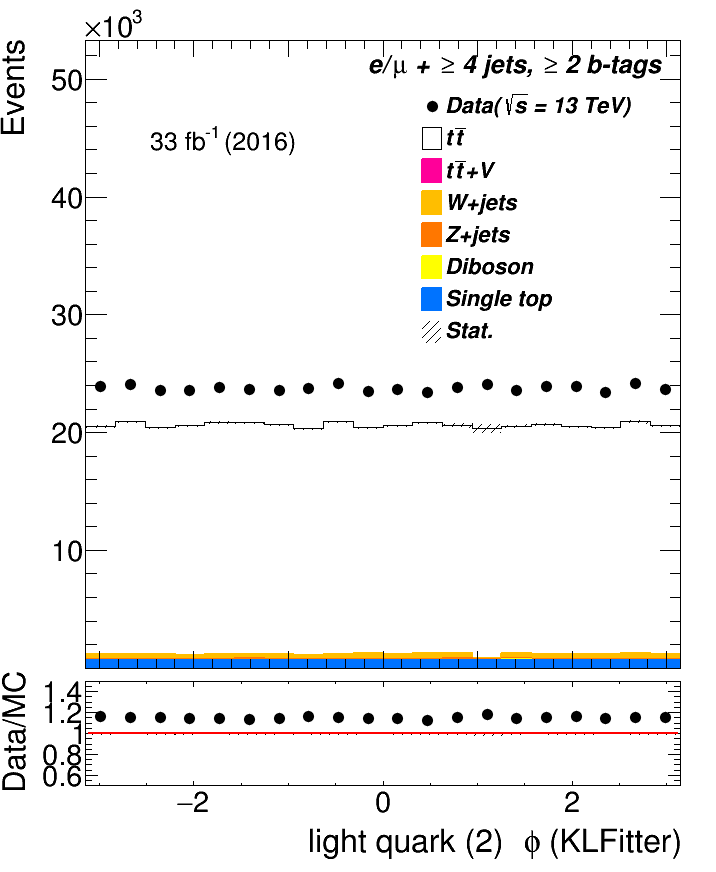
\includegraphics[width=\linewidth]{ControlPlots_emujets_2016_4incl_2incl/klf_lq2_phi_emujets_2016.png}
		\caption{$\phi$ of the second light jet.} \label{fig:klf14}
	\end{subfigure}	
	\hspace*{1.5cm}	
	\begin{subfigure}{0.35\textwidth}
		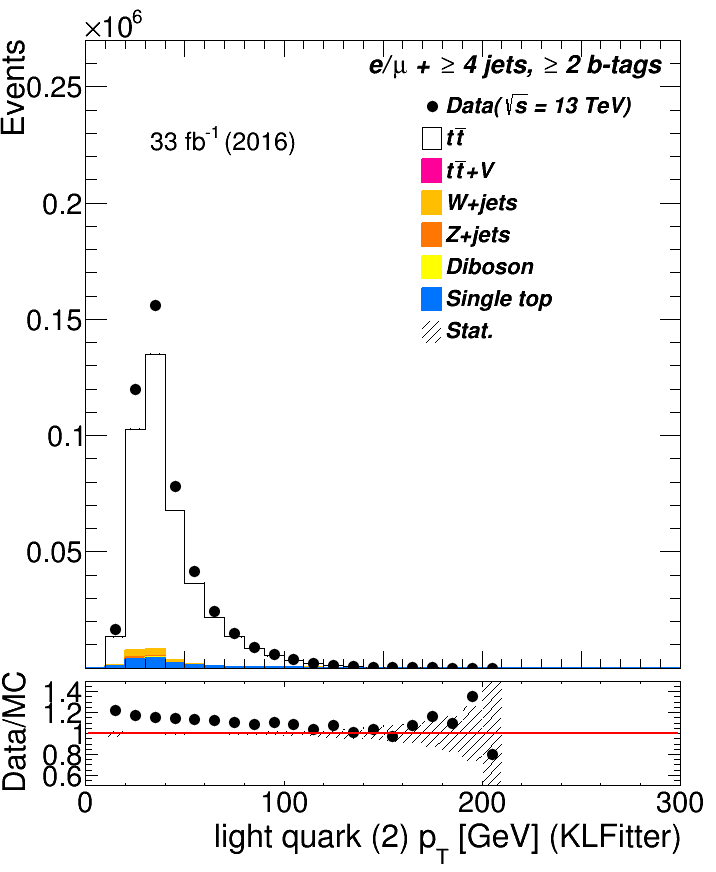
\includegraphics[width=\linewidth]{ControlPlots_emujets_2016_4incl_2incl/klf_lq2_pt_emujets_2016.png}
		\caption{Transverse momentum of the second light jet.} \label{fig:klf15}
	\end{subfigure}
	
	
	\medskip
	\begin{subfigure}{0.35\textwidth}
		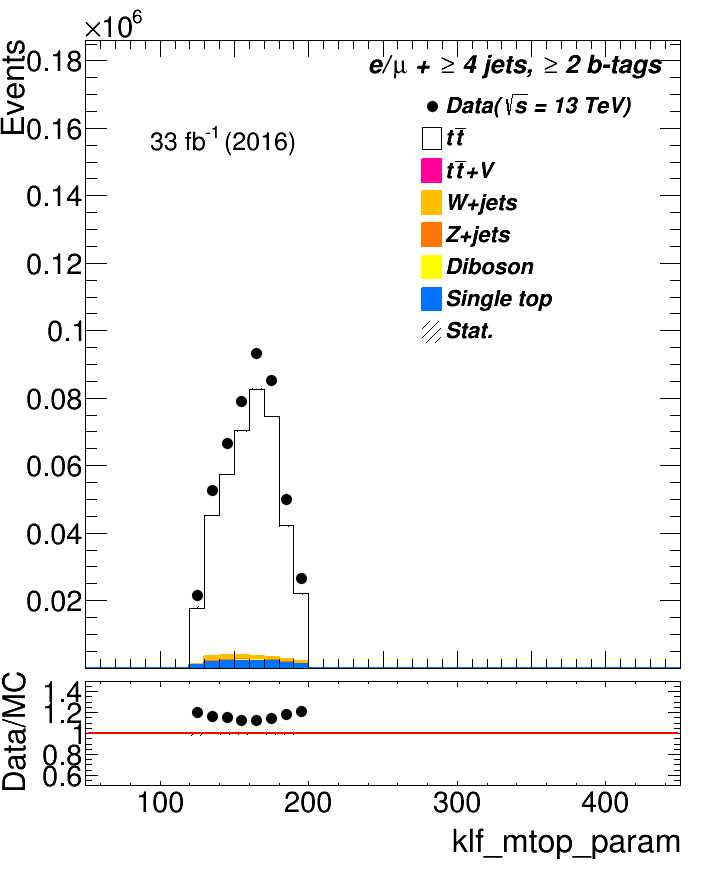
\includegraphics[width=\linewidth]{ControlPlots_emujets_2016_4incl_2incl/klf_mtop_param_emujets_2016.png}
		\caption{Hadronic top mass.} \label{fig:klf16}
	\end{subfigure}
	\hspace*{1.5cm}
	\begin{subfigure}{0.35\textwidth}
		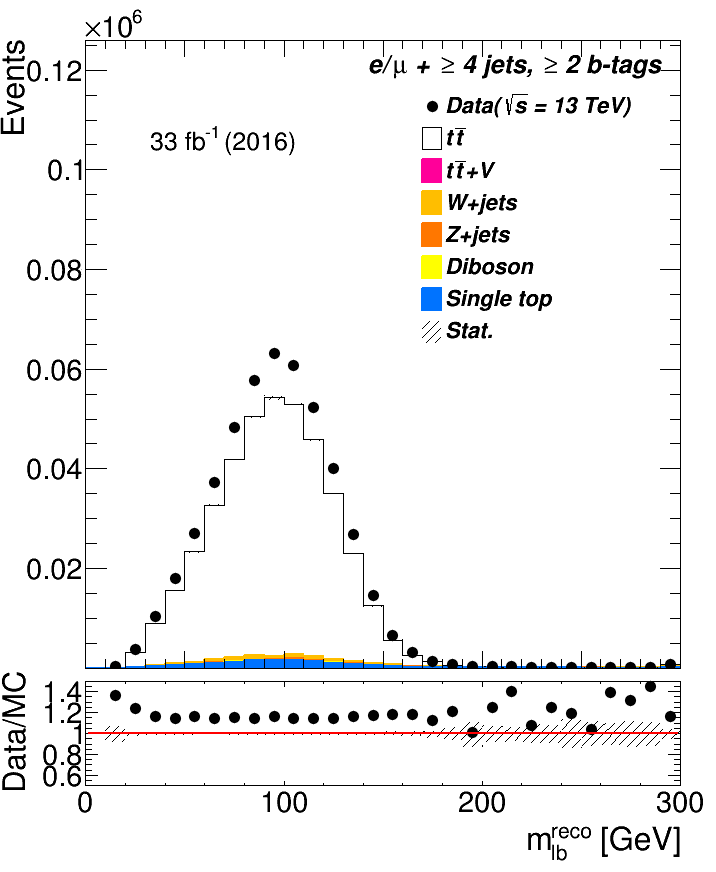
\includegraphics[width=\linewidth]{ControlPlots_emujets_2016_4incl_2incl/klf_original_mlb_reco_emujets_2016.png}
		\caption{Mass of the charged lepton and the leptonic $b$-jet.} \label{fig:klf17}
	\end{subfigure}
	
	
	\caption{bbbbbbbbbbbbbbbbbbbbbbbbbbbbbbbbbbbbbbbbbbbbbbbbbbbbbbbbbbbbbbbbbbbbbbbbbbb}
\end{figure}	




\begin{figure} % "[t!]" placement specifier just for this example
	\centering	
	\begin{subfigure}{0.35\textwidth}
		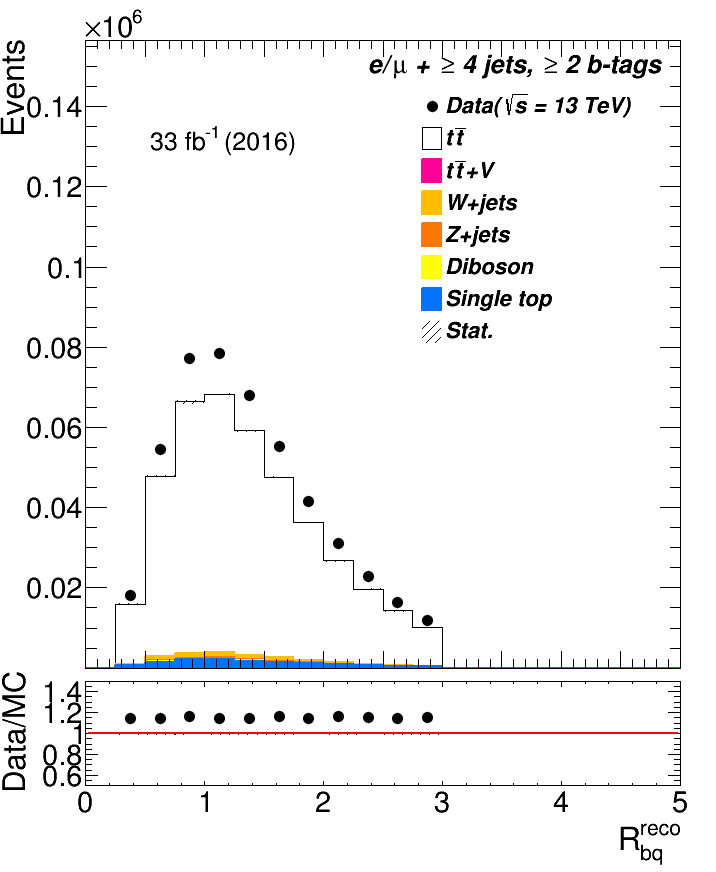
\includegraphics[width=\linewidth]{ControlPlots_emujets_2016_4incl_2incl/klf_original_Rbq_reco_emujets_2016.png}
		\caption{Ratio from reconstructed transvers momenta.} \label{fig:klf171}
	\end{subfigure}	
	\hspace*{1.5cm}	
	\begin{subfigure}{0.35\textwidth}
		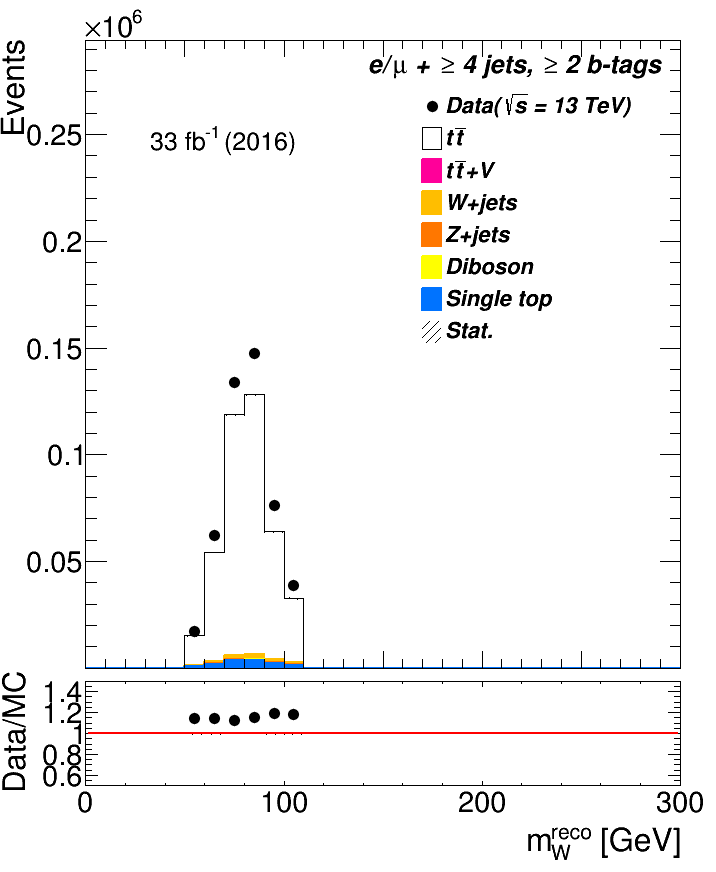
\includegraphics[width=\linewidth]{ControlPlots_emujets_2016_4incl_2incl/klf_original_Whad_m_emujets_2016.png}
		\caption{Hadronic $W$-boson mass.} \label{fig:18}
	\end{subfigure}
	\medskip	
	\begin{subfigure}{0.35\textwidth}
		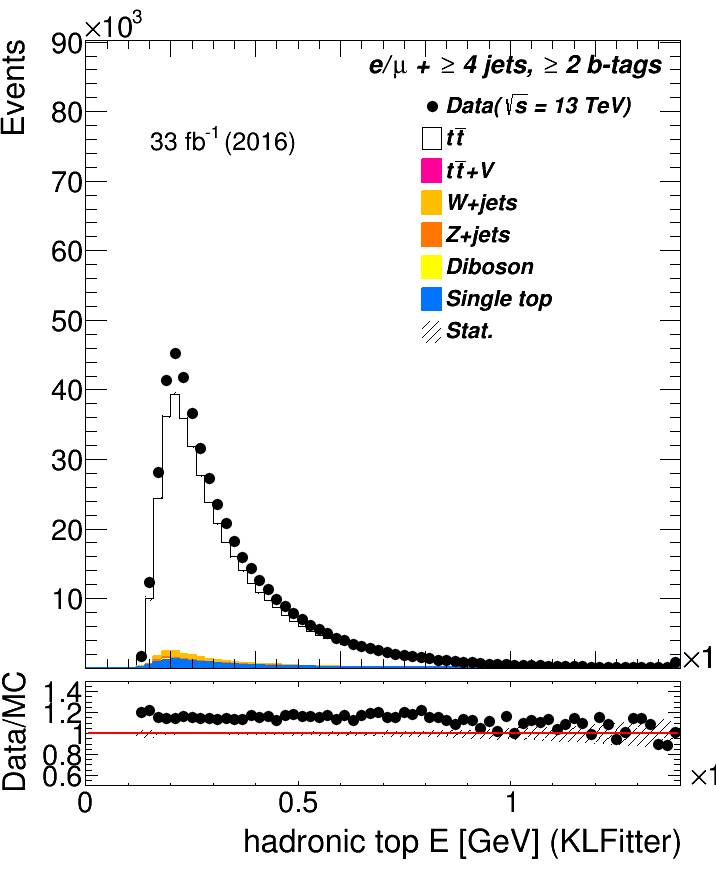
\includegraphics[width=\linewidth]{ControlPlots_emujets_2016_4incl_2incl/klf_topHad_E_emujets_2016.png}
		\caption{Hadronic top-quark energy.} \label{fig:19}
	\end{subfigure}
	\hspace*{1.5cm}	
	\begin{subfigure}{0.35\textwidth}
		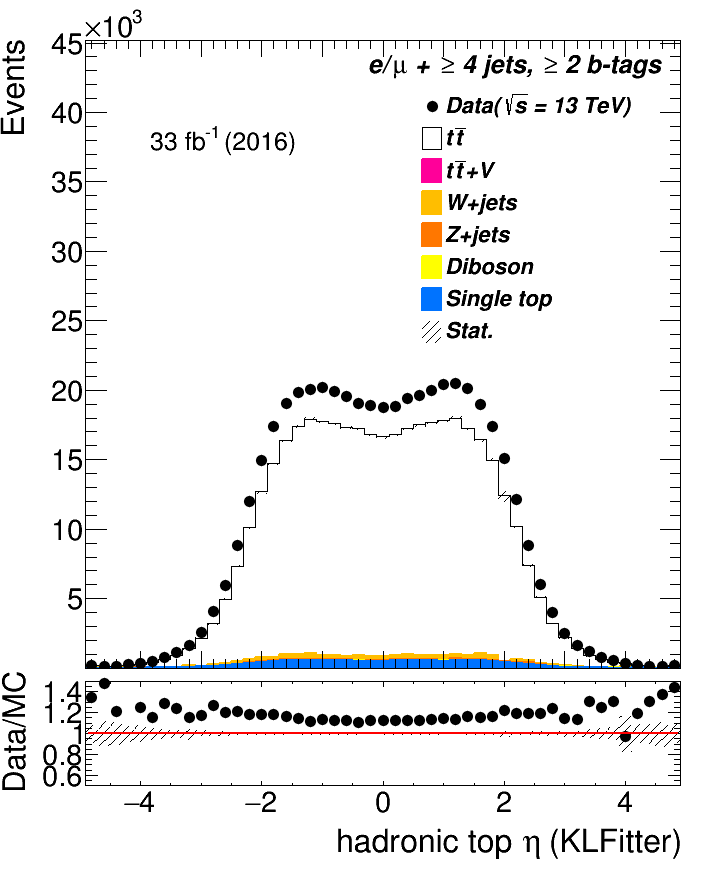
\includegraphics[width=\linewidth]{ControlPlots_emujets_2016_4incl_2incl/klf_topHad_eta_emujets_2016.png}
		\caption{Rapidity of the hadornic top-quark.} \label{fig:20}
	\end{subfigure}
	\medskip
	\begin{subfigure}{0.35\textwidth}
		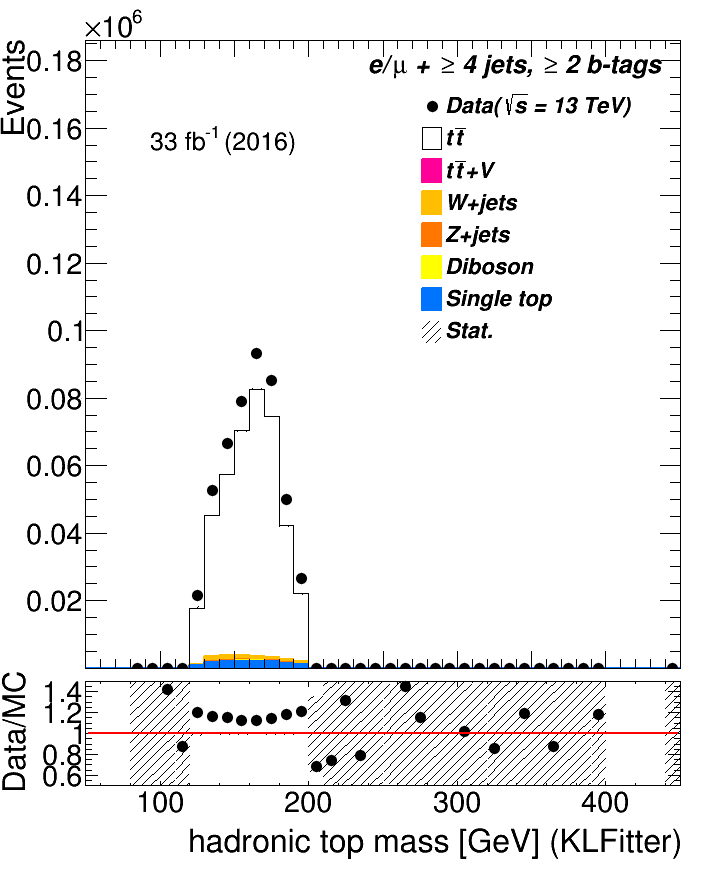
\includegraphics[width=\linewidth]{ControlPlots_emujets_2016_4incl_2incl/klf_topHad_m_emujets_2016.png}
		\caption{Hadronic top-quark mass.} \label{fig:21}
	\end{subfigure}	
	\hspace*{1.5cm}	
	\begin{subfigure}{0.35\textwidth}
		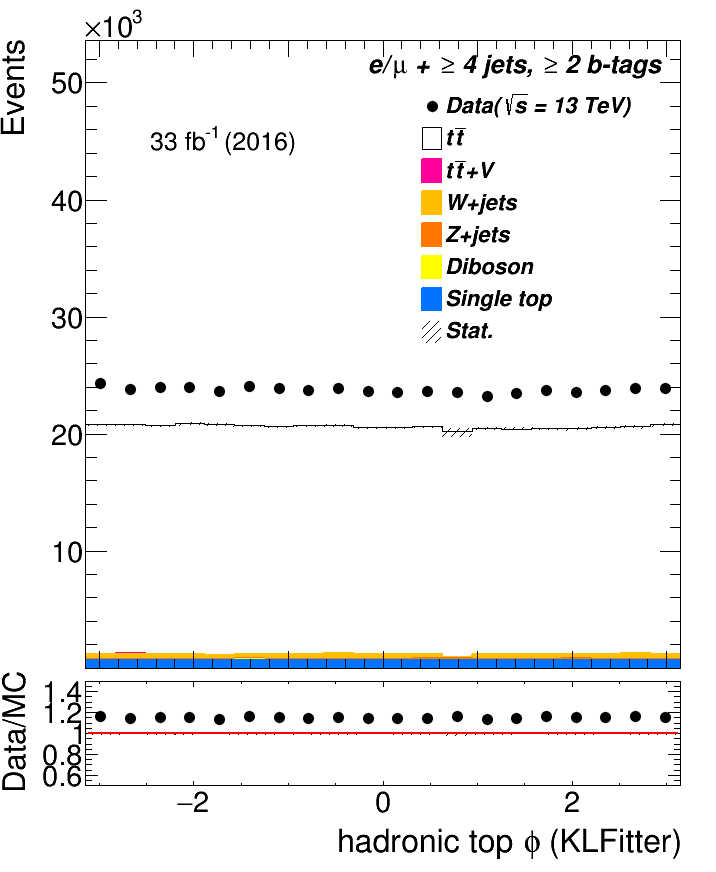
\includegraphics[width=\linewidth]{ControlPlots_emujets_2016_4incl_2incl/klf_topHad_phi_emujets_2016.png}
		\caption{$\phi$ of the hadronic top-quark.} \label{fig:22}
	\end{subfigure}
	\caption{bbbbbbbbbbbbbbbbbbbbbbbbbbbbbbbbbbbbbbbbbbbbbbbbbbbbbbbbbbbbbbbbbbbbbbbbbbb}
\end{figure}	








\begin{figure} % "[t!]" placement specifier just for this example
	\centering
	\begin{subfigure}{0.35\textwidth}
		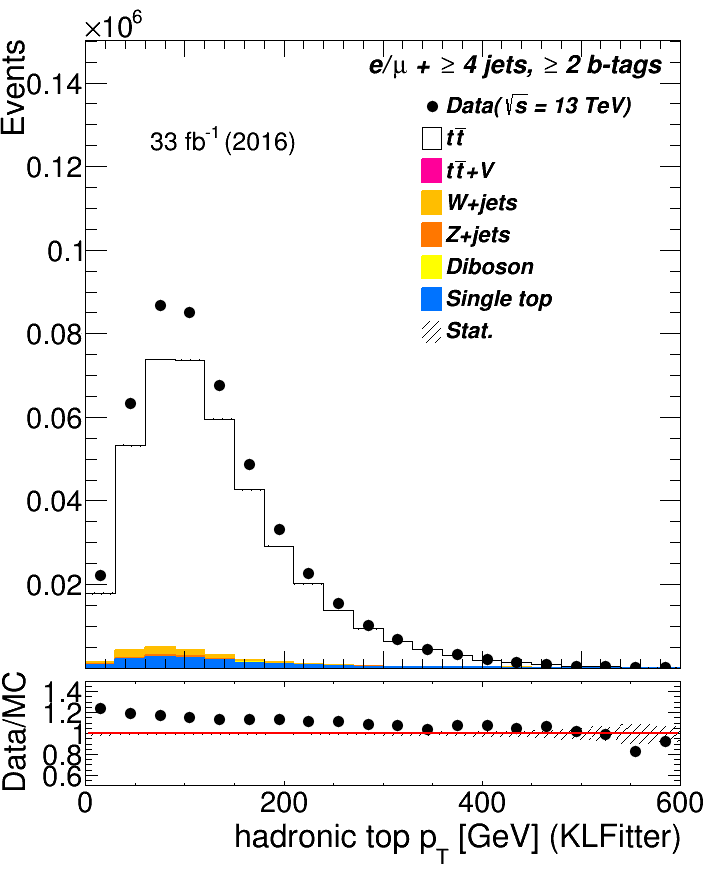
\includegraphics[width=\linewidth]{ControlPlots_emujets_2016_4incl_2incl/klf_topHad_pt_emujets_2016.png}
		\caption{Transverse momentum of the hadronic top-quark.} \label{fig:23}
	\end{subfigure}
	\hspace*{1.5cm}
	\begin{subfigure}{0.35\textwidth}
		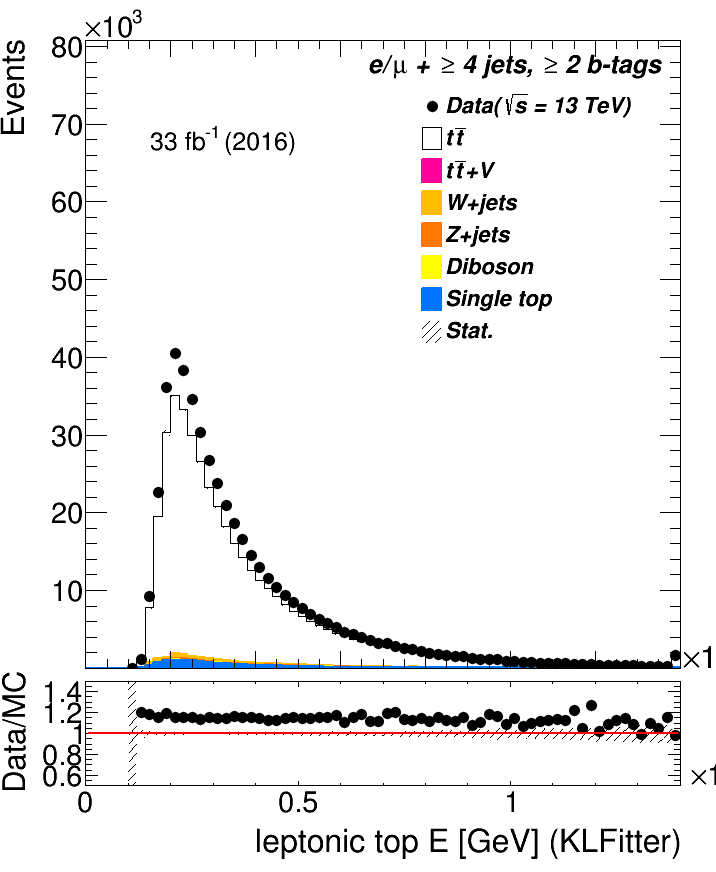
\includegraphics[width=\linewidth]{ControlPlots_emujets_2016_4incl_2incl/klf_topLep_E_emujets_2016.png}
		\caption{Leptonic top-quark energy.} \label{fig:24}
	\end{subfigure}
	\medskip	
	\begin{subfigure}{0.35\textwidth}
		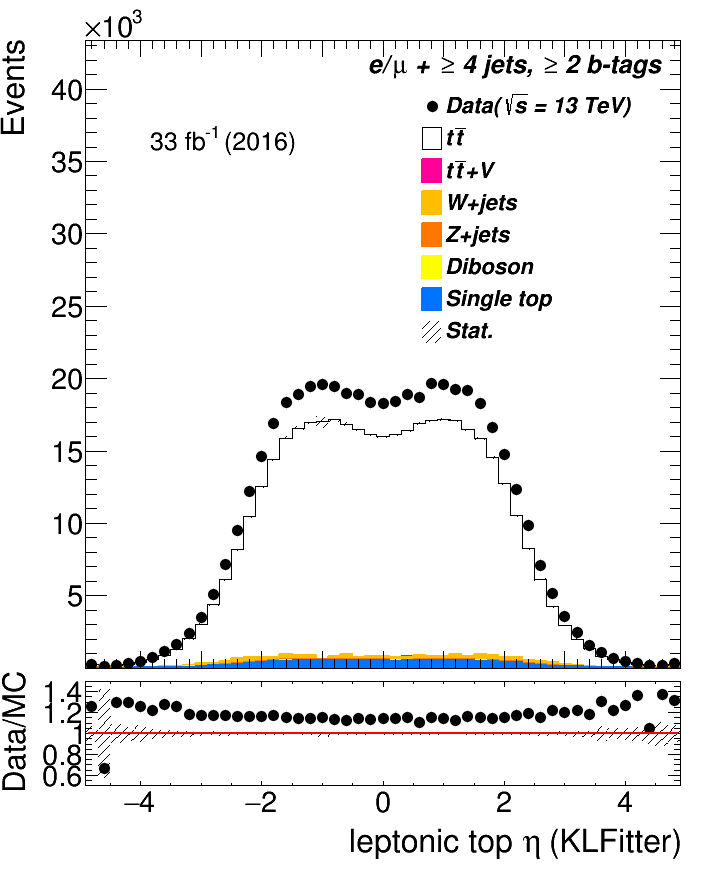
\includegraphics[width=\linewidth]{ControlPlots_emujets_2016_4incl_2incl/klf_topLep_eta_emujets_2016.png}
		\caption{Rapidty of the leptonic top-quark.} \label{fig:25}
	\end{subfigure}
	\hspace*{1.5cm}	
	\begin{subfigure}{0.35\textwidth}
		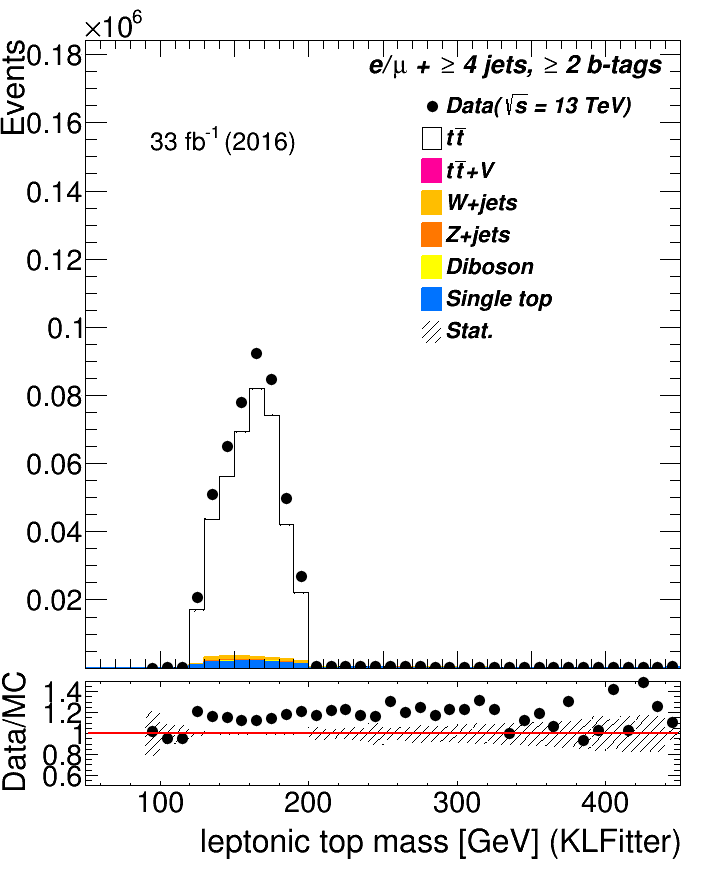
\includegraphics[width=\linewidth]{ControlPlots_emujets_2016_4incl_2incl/klf_topLep_m_emujets_2016.png}
		\caption{Mass of the leptoinc top-quark.} \label{fig:26}
	\end{subfigure}
	\medskip
	\begin{subfigure}{0.35\textwidth}
		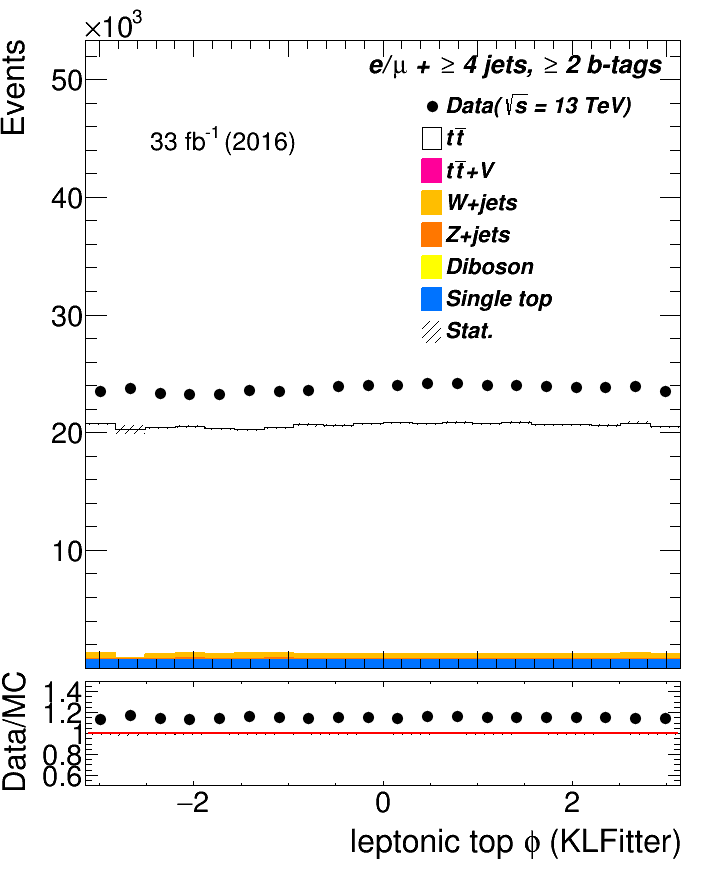
\includegraphics[width=\linewidth]{ControlPlots_emujets_2016_4incl_2incl/klf_topLep_phi_emujets_2016.png}
		\caption{$\phi$ of the leptonic top-quark.} \label{fig:27}
	\end{subfigure}
	\hspace*{1.5cm}
	\begin{subfigure}{0.35\textwidth}
		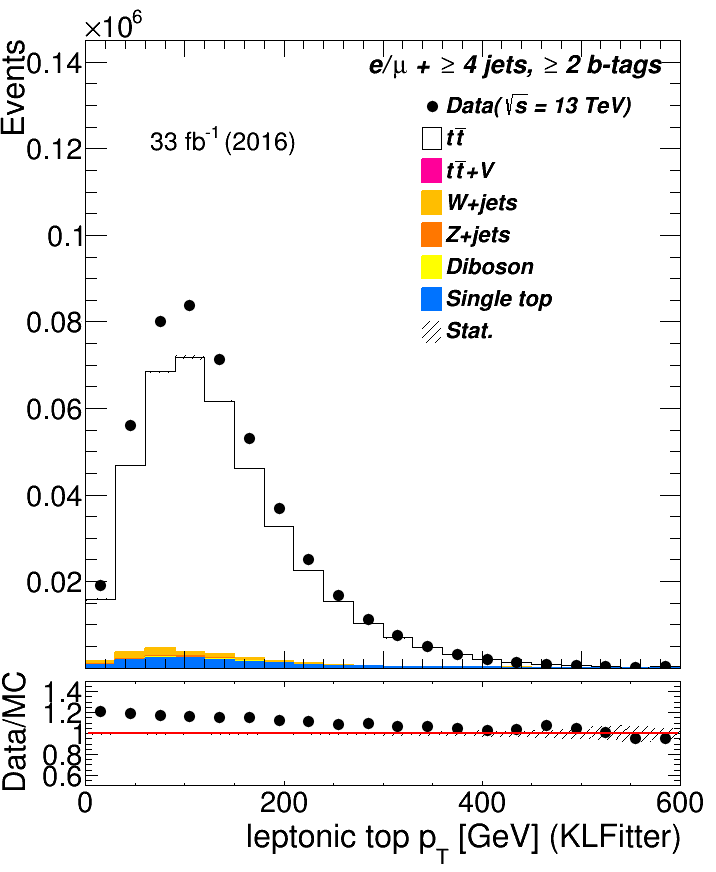
\includegraphics[width=\linewidth]{ControlPlots_emujets_2016_4incl_2incl/klf_topLep_pt_emujets_2016.png}
		\caption{Transverse momentum of the leptonic top-quark.} \label{fig:28}
	\end{subfigure}	
	\caption{bbbbbbbbbbbbbbbbbbbbbbbbbbbbbbbbbbbbbbbbbbbbbbbbbbbbbbbbbbbbbbbbbbbbbbbbbbb}
\end{figure}	


\begin{figure} % "[t!]" placement specifier just for this example
	\centering
	\begin{subfigure}{0.35\textwidth}
		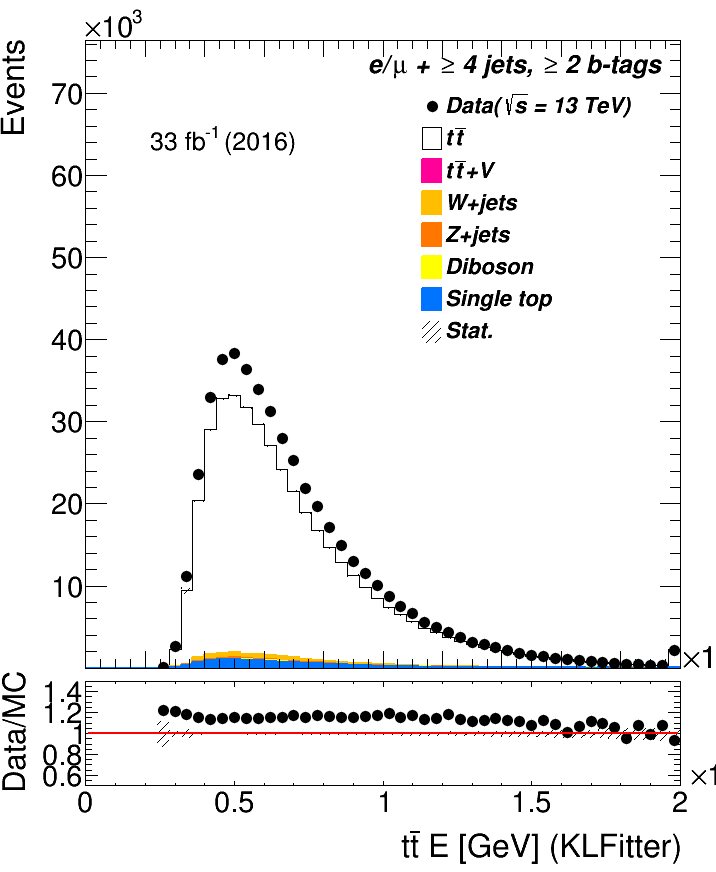
\includegraphics[width=\linewidth]{ControlPlots_emujets_2016_4incl_2incl/klf_ttbar_E_emujets_2016.png}
		\caption{Energy of the top-quark pair.} \label{fig:29}
	\end{subfigure}
	\hspace*{1.5cm}
	\begin{subfigure}{0.35\textwidth}
		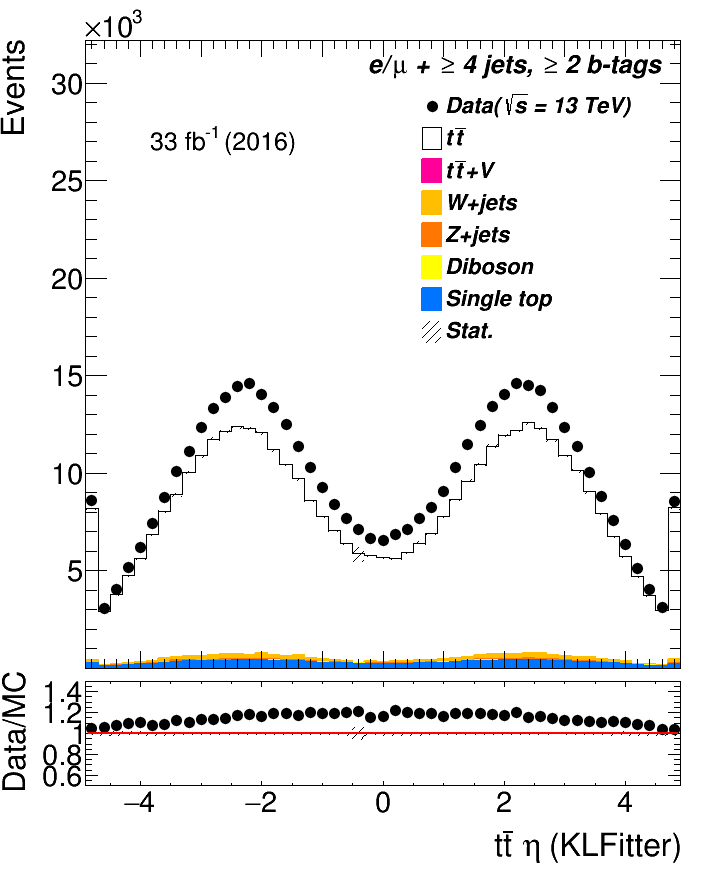
\includegraphics[width=\linewidth]{ControlPlots_emujets_2016_4incl_2incl/klf_ttbar_eta_emujets_2016.png}
		\caption{Rapidity of the top-quark pair.} \label{fig:30}
	\end{subfigure}
	\medskip
	\begin{subfigure}{0.35\textwidth}
		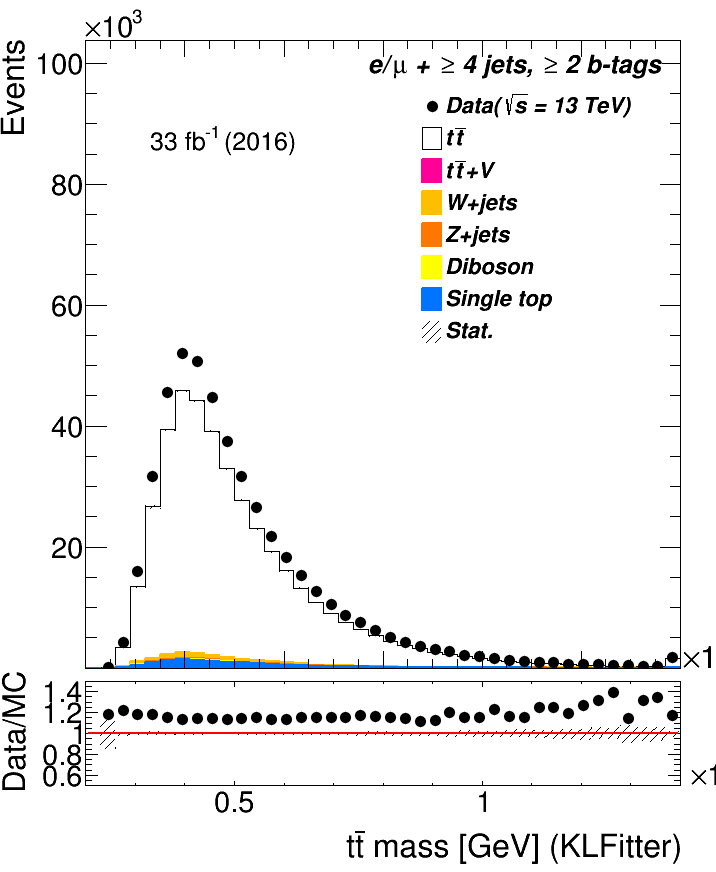
\includegraphics[width=\linewidth]{ControlPlots_emujets_2016_4incl_2incl/klf_ttbar_m_emujets_2016.png}
		\caption{Mass of the top-quark pair.} \label{fig:31}
	\end{subfigure}
	\hspace*{1.5cm}
	\begin{subfigure}{0.35\textwidth}
		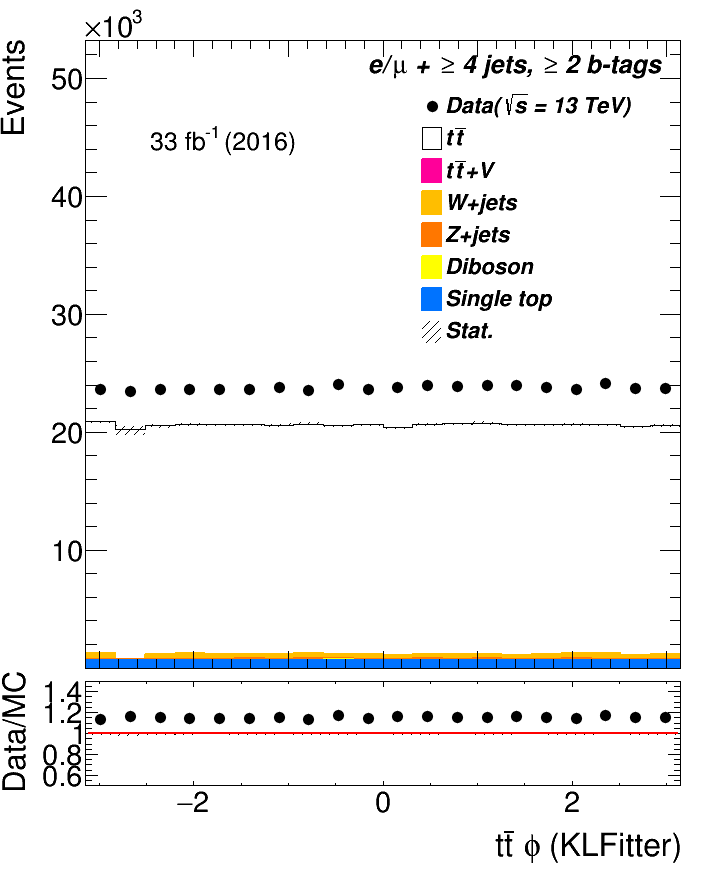
\includegraphics[width=\linewidth]{ControlPlots_emujets_2016_4incl_2incl/klf_ttbar_phi_emujets_2016.png}
		\caption{$\phi$ of the top-quark pair.} \label{fig:32}
	\end{subfigure}
	\medskip
	\begin{subfigure}{0.35\textwidth}
		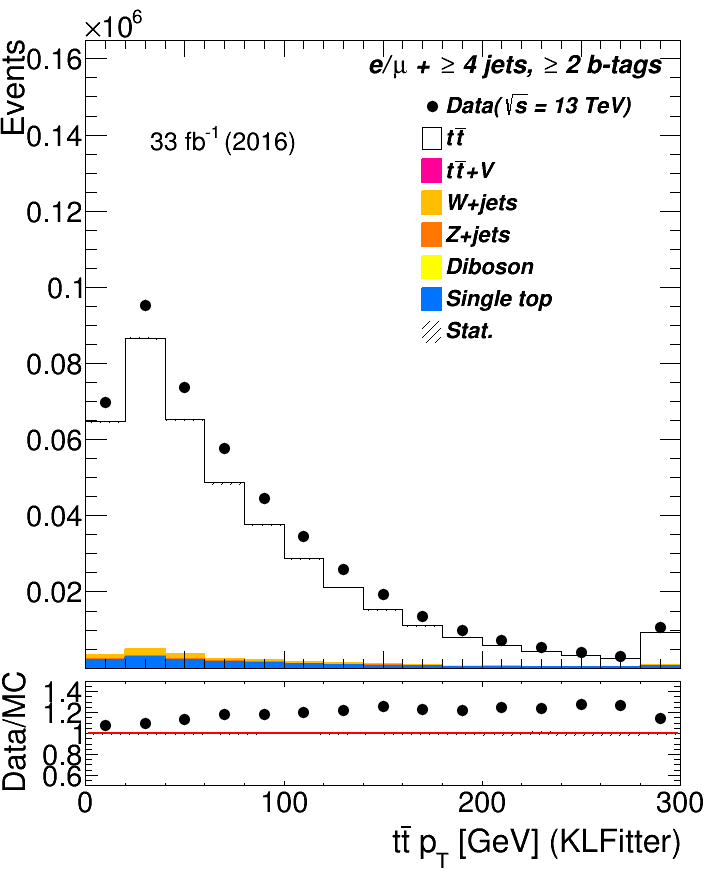
\includegraphics[width=\linewidth]{ControlPlots_emujets_2016_4incl_2incl/klf_ttbar_pt_emujets_2016.png}
		\caption{Transverse momentum of the top-quark pair.} \label{fig:33}
	\end{subfigure}
	\hspace*{1.5cm}	
	\begin{subfigure}{0.35\textwidth}
		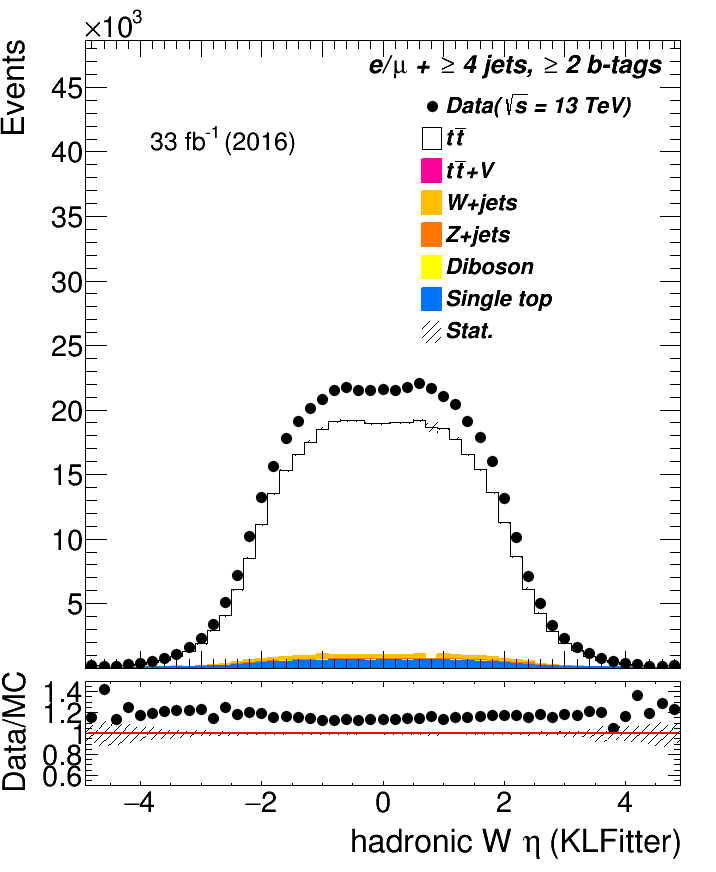
\includegraphics[width=\linewidth]{ControlPlots_emujets_2016_4incl_2incl/klf_Whad_eta_emujets_2016.png}
		\caption{Rapidty of the hadronic $W$-boson.} \label{fig:34}
	\end{subfigure}
	\caption{bbbbbbbbbbbbbbbbbbbbbbbbbbbbbbbbbbbbbbbbbbbbbbbbbbbbbbbbbbbbbbbbbbbbbbbbbbb}
\end{figure}	








\begin{figure} % "[t!]" placement specifier just for this example
	\centering
	\begin{subfigure}{0.35\textwidth}
		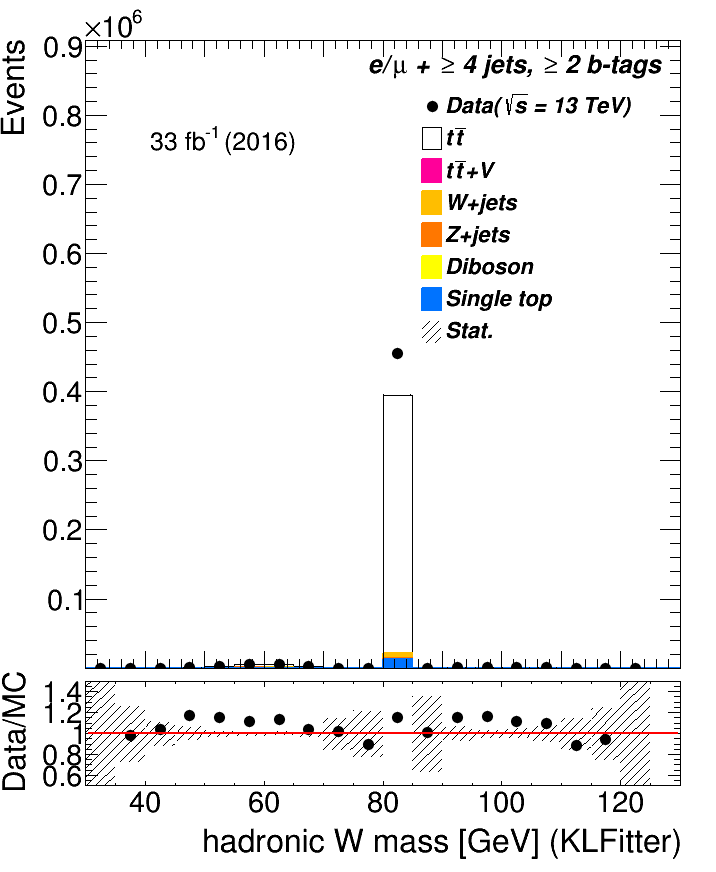
\includegraphics[width=\linewidth]{ControlPlots_emujets_2016_4incl_2incl/klf_Whad_m_emujets_2016.png}
		\caption{Hadronic $W$-boson mass.} \label{fig:35}
	\end{subfigure}
	\hspace*{1.5cm}
	\begin{subfigure}{0.35\textwidth}
		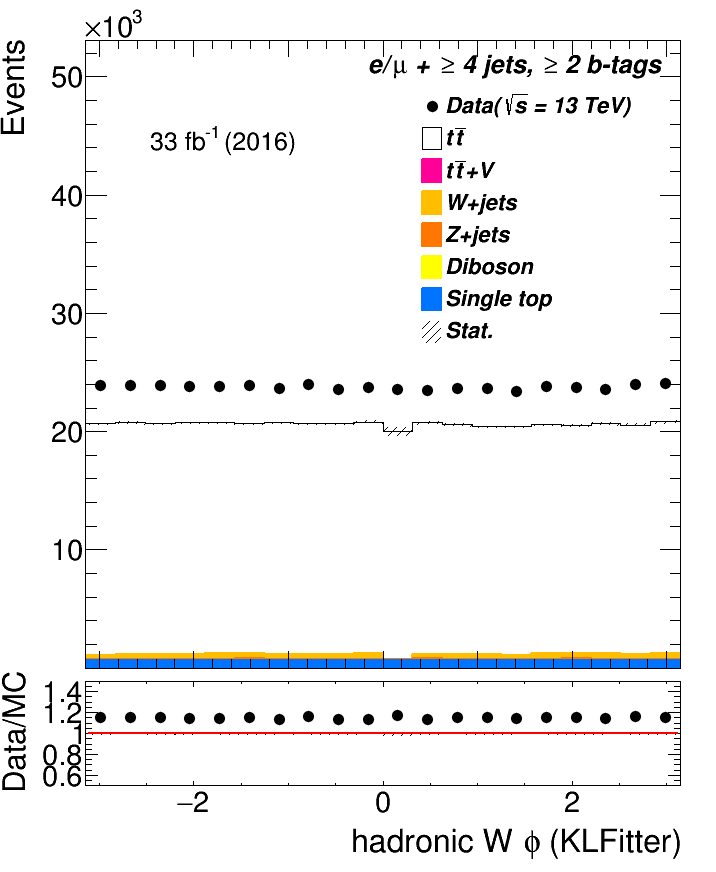
\includegraphics[width=\linewidth]{ControlPlots_emujets_2016_4incl_2incl/klf_Whad_phi_emujets_2016.png}
		\caption{$\phi$ of the hadronic $W$-boson.} \label{fig:36}
	\end{subfigure}
	\medskip
	\begin{subfigure}{0.35\textwidth}
		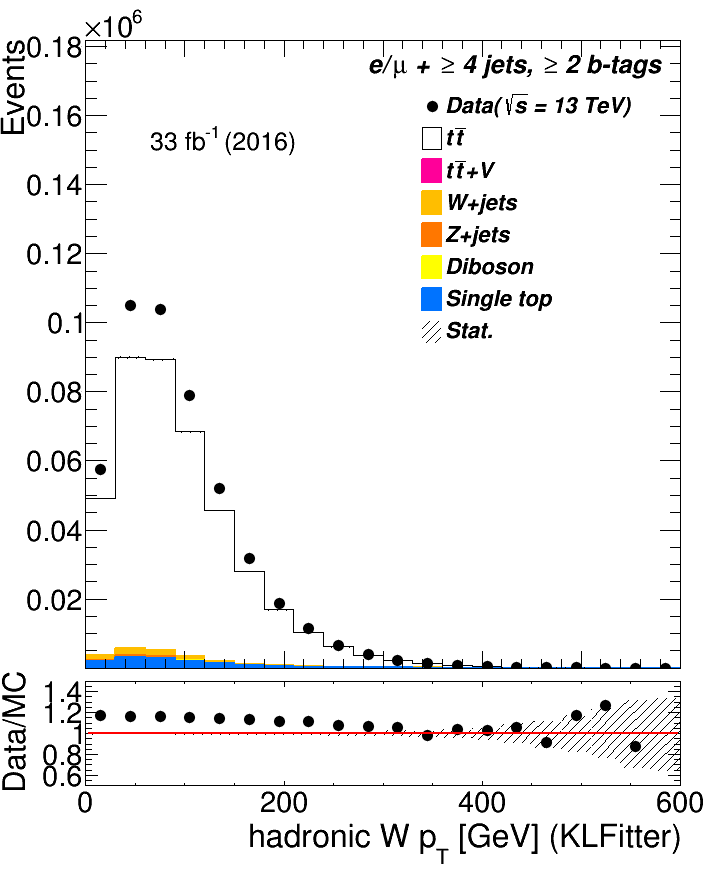
\includegraphics[width=\linewidth]{ControlPlots_emujets_2016_4incl_2incl/klf_Whad_pt_emujets_2016.png}
		\caption{Transverse mementom of the hadronic $W$-boson.} \label{fig:37}
	\end{subfigure}
	\hspace*{1.5cm}	
	\begin{subfigure}{0.35\textwidth}
		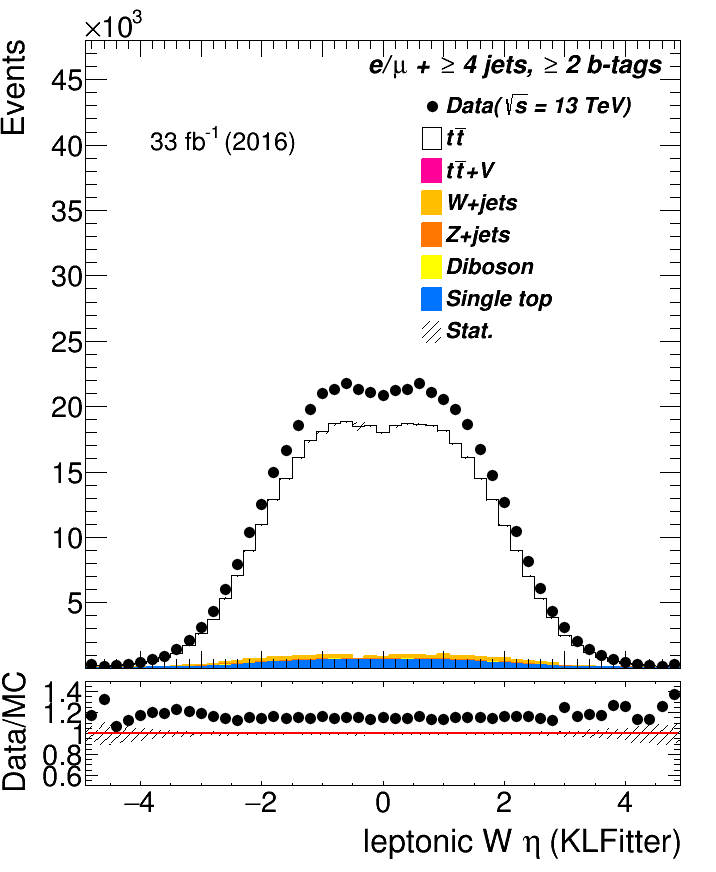
\includegraphics[width=\linewidth]{ControlPlots_emujets_2016_4incl_2incl/klf_Wlep_eta_emujets_2016.png}
		\caption{Rapidity of the leptonic $W$-boson.} \label{fig:38}
	\end{subfigure}
	\medskip	
	\begin{subfigure}{0.35\textwidth}
		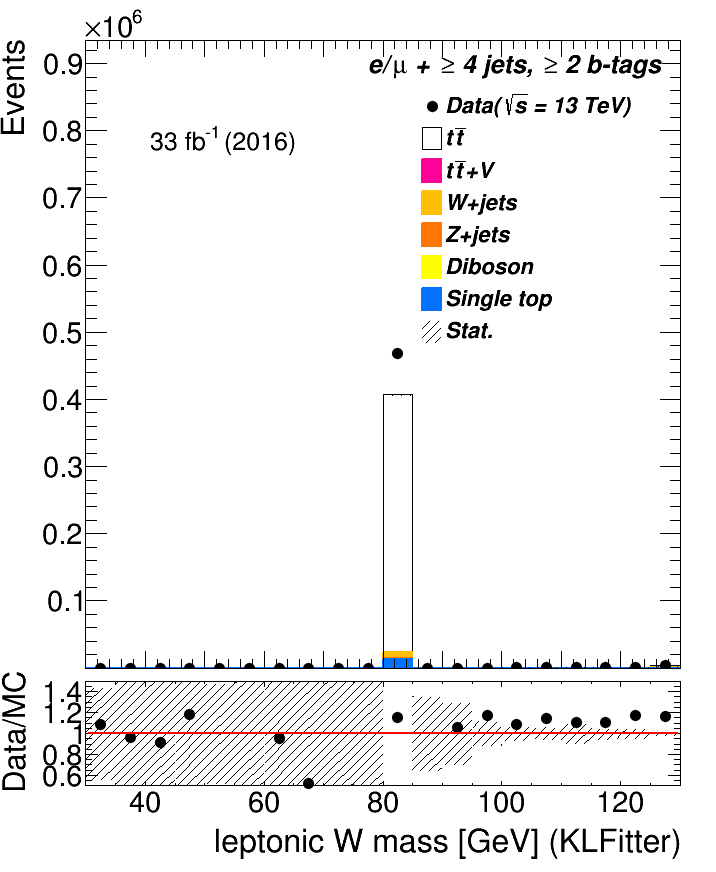
\includegraphics[width=\linewidth]{ControlPlots_emujets_2016_4incl_2incl/klf_Wlep_m_emujets_2016.png}
		\caption{Mass of the leptonic $W$-boson mass.} \label{fig:39}
	\end{subfigure}
	\hspace*{1.5cm}
	\begin{subfigure}{0.35\textwidth}
		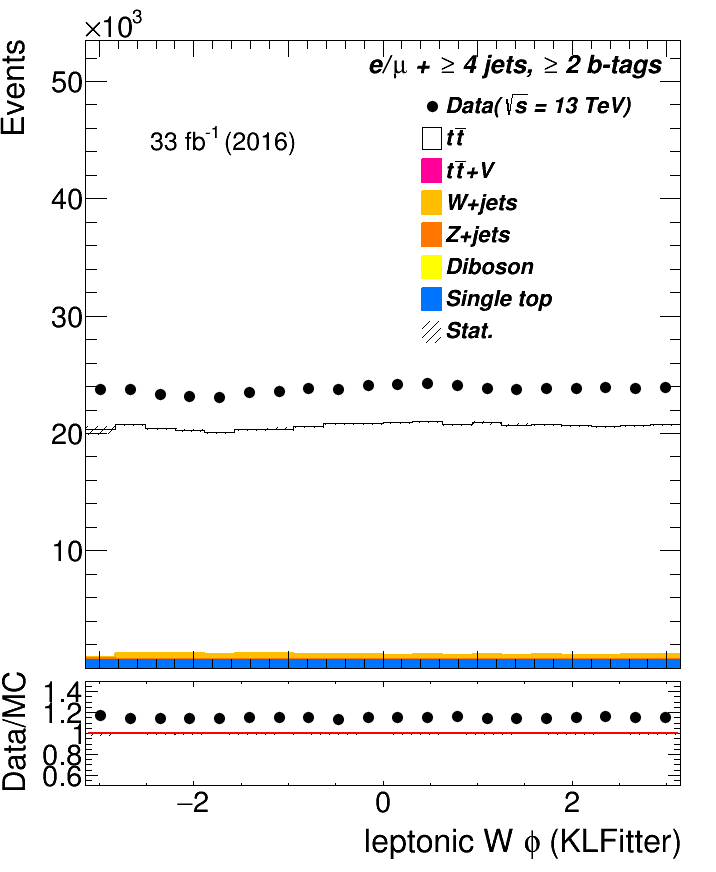
\includegraphics[width=\linewidth]{ControlPlots_emujets_2016_4incl_2incl/klf_Wlep_phi_emujets_2016.png}
		\caption{$\phi$ of the leptonic $W$-boson.} \label{fig:40}
	\end{subfigure}
	\caption{bbbbbbbbbbbbbbbbbbbbbbbbbbbbbbbbbbbbbbbbbbbbbbbbbbbbbbbbbbbbbbbbbbbbbbbbbbb}
\end{figure}	



\begin{figure} % "[t!]" placement specifier just for this example
	\centering
	
	\begin{subfigure}{0.35\textwidth}
		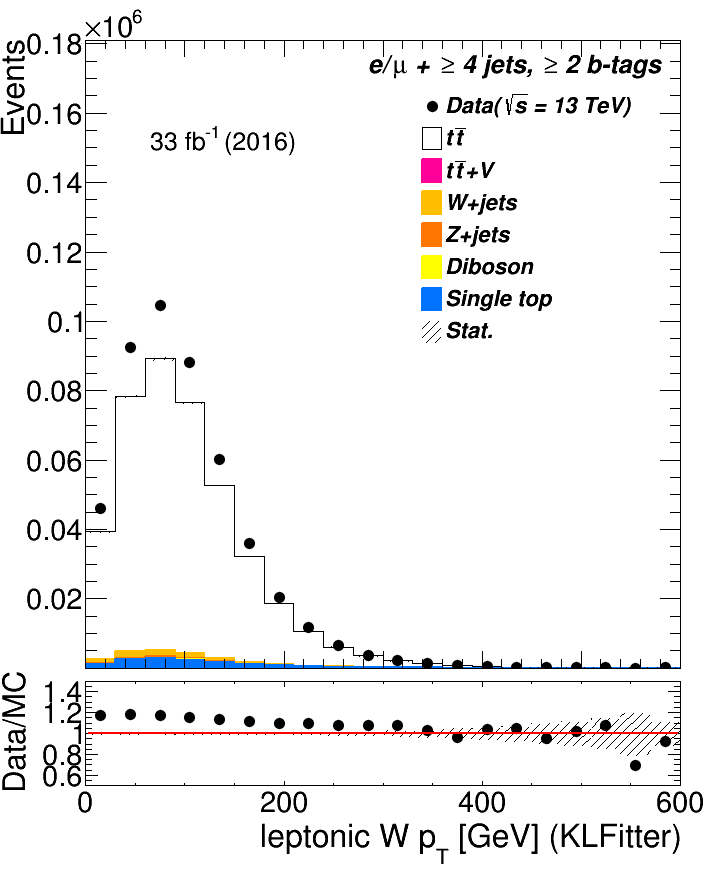
\includegraphics[width=\linewidth]{ControlPlots_emujets_2016_4incl_2incl/klf_Wlep_pt_emujets_2016.png}
		\caption{Transverse momentum of the leptonic $W$-boson.} \label{fig:411}
	\end{subfigure}
	\hspace*{1.5cm}
	\begin{subfigure}{0.35\textwidth}
		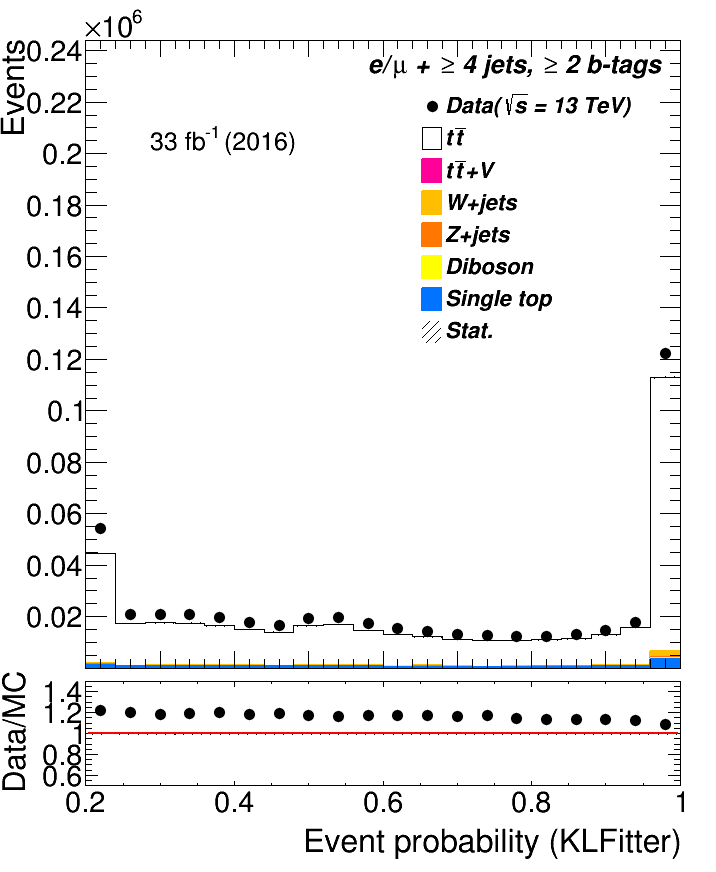
\includegraphics[width=\linewidth]{ControlPlots_emujets_2016_4incl_2incl/klf_eventProbability_emujets_2016.png}
		\caption{Event probability.} \label{fig:422}
	\end{subfigure}
	\medskip
	\begin{subfigure}{0.35\textwidth}
		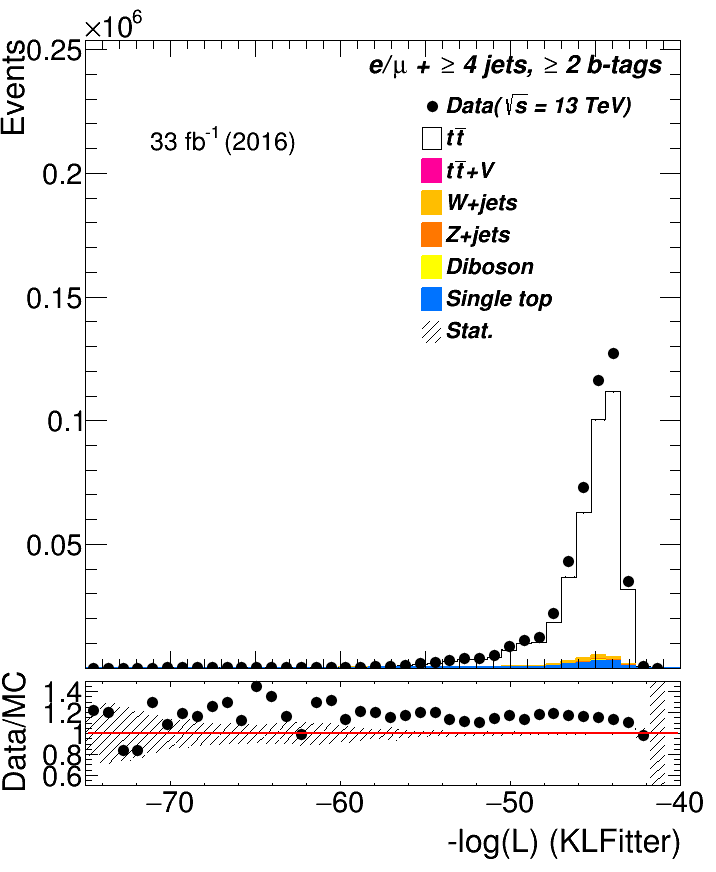
\includegraphics[width=\linewidth]{ControlPlots_emujets_2016_4incl_2incl/klf_LL_emujets_2016.png}
		\caption{\textsc{KLFitter} likelihood.} \label{fig:433}
	\end{subfigure}	
	\hspace*{1.5cm}	
	\begin{subfigure}{0.35\textwidth}
		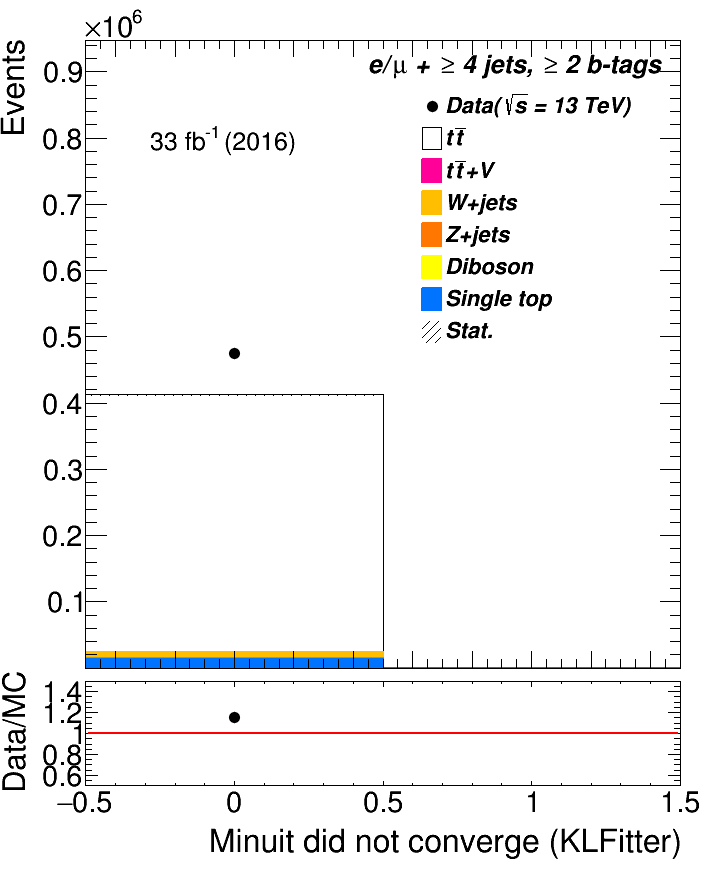
\includegraphics[width=\linewidth]{ControlPlots_emujets_2016_4incl_2incl/klf_minuitDidNotConverge_emujets_2016.png}
		\caption{\textsc{MINUIT} did not converge.} \label{fig:444}
	\end{subfigure}
	
	
	\caption{bbbbbbbbbbbbbbbbbbbbbbbbbbbbbbbbbbbbbbbbbbbbbbbbbbbbbbbbbbbbbbbbbbbbbbbbbbb}
\end{figure}	








